\documentclass{article}
%\usepackage[english]{babel}%
\usepackage[dvipsnames]{xcolor}
\usepackage{graphicx}
\usepackage{tabulary}
\usepackage{tabularx}
\usepackage[normalem]{ulem}
\usepackage{cancel}
\usepackage{tikz} 
\usepackage{tikz-3dplot}
\usepgflibrary{shapes.geometric}
\usepackage{pdflscape}
\usetikzlibrary{shapes.multipart, shapes.geometric, arrows}
\usepackage{colortbl}
\usepackage{chemplants}
\usepackage{lastpage}
\usepackage{multirow}
\usepackage{enumerate}
\usepackage{color,soul}
\usepackage{pdflscape}
\usepackage{hyperref}
%\usepackage[table]{xcolor}
\usepackage{rotating}
\usepackage{amsmath}
\usepackage{fixltx2e}
\usepackage{framed}
\usepackage{mdframed}
\usepackage[T1]{fontenc}
\usepackage[utf8]{inputenc}
\usepackage{textcomp}
\usepackage{siunitx}
\usepackage{ifthen}
\usepackage{fancyhdr}
\usepackage{gensymb}
 \usepackage{newunicodechar}

 \usepackage{pgfplots}
\usepackage[document]{ragged2e}
\usetikzlibrary{positioning}
\usetikzlibrary{decorations.pathreplacing}
\usetikzlibrary{automata}
\usetikzlibrary {shapes.multipart}
\usepackage{pstricks}
\usepackage[margin=1in,top=1.2in,headheight=57pt,headsep=0.1in]
{geometry}

 \usepackage{ifthen}
\usepackage{fancyhdr}
\everymath{\displaystyle}
\usepackage[document]{ragged2e}
\usepackage{fancyhdr}
\everymath{\displaystyle}
\usetikzlibrary{calc}
\usetikzlibrary{arrows}
\linespread{2}%controls the spacing between lines. Bigger fractions means crowded lines%
%\pagestyle{fancy}
%\usepackage[margin=1 in, top=1in, includefoot]{geometry}
%\everymath{\displaystyle}
\linespread{1.3}%controls the spacing between lines. Bigger fractions means crowded lines%
%\pagestyle{fancy}
\pagestyle{fancy}
\setlength{\headheight}{56.2pt}


\chead{\ifthenelse{\value{page}=1}{
\includegraphics[scale=0.3]{SCC}\\ \textbf \textbf Final Exam}}
\rhead{\ifthenelse{\value{page}=1}{Shabbir Basrai}{Shabbir Basrai}}
\lhead{\ifthenelse{\value{page}=1}{WATR 081 - Spring 2022}{\textbf Final Exam}}
\rfoot{\ifthenelse{\value{page}=1}{}{WATR 081 - Spring 2022}}

\cfoot{}
\lfoot{Page \thepage\ of \pageref{LastPage}}
\renewcommand{\headrulewidth}{2pt}
\renewcommand{\footrulewidth}{1pt}
\begin{document}

\begin{tikzpicture}
\draw (0,0) ellipse (0.1cm and 0.3cm);
\draw (10,0) ellipse (0.1cm and 0.3cm);
\draw [-] (0,-0.29) -- (10,-0.29);
\draw [-] (0,0.29) -- (10,0.29);
\draw [<->] (10,-0.28) -- (10,0.28) node [midway, below=-3mm] {\hspace{2.6cm}Diameter=6"};
\draw [<->] (0,-.68) -- (10,-.68)node [midway, below] {\hspace{0.9cm}Length=1,200'};
\end{tikzpicture}

\begin{tikzpicture}[mydashed/.style={dashed,dash phase=2pt}]
\draw (0,0) ellipse (2cm and 0.3cm) node [midway, above=-2.4mm] {};
\draw (0,-2.3) ellipse (2cm and 0.3cm) node [midway, below=2.05cm] {};
\draw [-] (2,-2.3) -- (2,0);
%\draw [<->] (-2,0) -- (2,0); 
\draw [<->] (2.5,-2.3) -- (2.5,0) node [midway, below] {\hspace{2.9cm}Height (h) = 25'};
\draw [<->] (-2,-0.4) -- (2,-0.4) node [midway, below=0.7mm] {\hspace{0.1cm}\small{Diameter (D)}=80'};
%\draw [-] (0,-4) -- (2,-2.3);
%\draw [-] (0,-4) -- (-2,-2.3);
%\draw [-] (0,-4) -- (2,-2.3);
\draw [-] (-2,0) -- (-2,-2.3) node [midway, below] {\hspace{4cm}\tiny{Cylinder Surface Area$=\pi*D*h$}};
\draw [-latex, mydashed, line width=1mm, rotate=-90] (0.6,-1.9) arc [start angle=-120, end angle=120, x radius=0.8cm, y radius=2.2cm];
%\draw [-latex, thick, rotate=-95] (0,0) arc [start angle=-190, end angle=160, x radius=1cm, y radius=2cm];
\end{tikzpicture}

\begin{tikzpicture}
\draw (0,0) ellipse (2.1cm and 0.7cm);
\draw (0,-2) ellipse (2.1cm and 0.7cm);
%\draw [-] (0,-0.29) -- (10,-0.29);
%\draw [-] (0,0.29) -- (10,0.29);
%\draw [<->] (10,-0.28) -- (10,0.28) node [midway, below=-3mm] {\hspace{2.6cm}Diameter=6"};
%\draw [<->] (0,-.68) -- (10,-.68)node [midway, below] {\hspace{0.9cm}Length=1,200'};
\end{tikzpicture}


\vspace{1cm}



\begin{tikzpicture}
	%%% Edit the following coordinate to change the shape of your
	%%% cuboid
      
	%% Vanishing points for perspective handling
	\coordinate (P1) at (-7cm,1.5cm); % left vanishing point (To pick)
	\coordinate (P2) at (8cm,1.5cm); % right vanishing point (To pick)

	%% (A1) and (A2) defines the 2 central points of the cuboid
	\coordinate (A1) at (0em,0cm); % central top point (To pick)
	\coordinate (A2) at (0em,-2cm); % central bottom point (To pick)

	%% (A3) to (A8) are computed given a unique parameter (or 2) .8
	% You can vary .8 from 0 to 1 to change perspective on left side
	\coordinate (A3) at ($(P1)!.8!(A2)$); % To pick for perspective 
	\coordinate (A4) at ($(P1)!.8!(A1)$);

	% You can vary .8 from 0 to 1 to change perspective on right side
	\coordinate (A7) at ($(P2)!.7!(A2)$);
	\coordinate (A8) at ($(P2)!.7!(A1)$);

	%% Automatically compute the last 2 points with intersections
	\coordinate (A5) at
	  (intersection cs: first line={(A8) -- (P1)},
			    second line={(A4) -- (P2)});
	\coordinate (A6) at
	  (intersection cs: first line={(A7) -- (P1)}, 
			    second line={(A3) -- (P2)});

	%%% Depending of what you want to display, you can comment/edit
	%%% the following lines

	%% Possibly draw back faces

	\fill[gray!40] (A2) -- (A3) -- (A6) -- (A7) -- cycle; % face 6
	\node at (barycentric cs:A2=1,A3=1,A6=1,A7=1) {};
	
	\fill[gray!50] (A3) -- (A4) -- (A5) -- (A6) -- cycle; % face 3
	\node at (barycentric cs:A3=1,A4=1,A5=1,A6=1) {\tiny Wall - W*H};
	
	\fill[gray!10, opacity=0.2] (A5) -- (A6) -- (A7) -- (A8) -- cycle; % face 4
	\node at (barycentric cs:A5=1,A6=1,A7=1,A8=1) {\tiny Wall - L*H};
	
	\fill[gray!10,opacity=0.5] (A1) -- (A2) -- (A3) -- (A4) -- cycle; % f2
	\node at (barycentric cs:A1=1,A2=1,A3=1,A4=1) {\tiny Wall - L*H};
	
	\fill[gray!40,opacity=0.2] (A1) -- (A4) -- (A5) -- (A8) -- cycle; % f5
	\node at (barycentric cs:A1=1,A4=1,A5=1,A8=1) {};	
	
	\draw[thick,dashed] (A5) -- (A6);
	\draw[thick,dashed] (A3) -- (A6);
	\draw[thick,dashed] (A7) -- (A6);

	%% Possibly draw front faces

	%\fill[orange] (A1) -- (A8) -- (A7) -- (A2) -- cycle; % face 1
	\node at (barycentric cs:A1=1,A8=1,A7=1,A2=1) {\tiny Wall - W*H};
	


	%% Possibly draw front lines
	\draw[thick] (A1) -- (A2);

	\draw[<->] (-1.8,0.38) -- (-1.8,-1.3)node [midway, above=-1.8mm] {\hspace{-1.3cm}\tiny Height=20'};
	\draw[<->] (-1.6,-1.4) -- (-.3,-2.1)node [midway, above=-2.6mm] {\hspace{-1.3cm}\tiny Length=45'};
	\draw[<->] (2.6,-1.13) -- (0.2,-2.2)node [midway, below=.6mm] {\hspace{1.2cm}\tiny Width=65'};
	\draw[thick] (A3) -- (A4);
	\draw[thick] (A7) -- (A8);
	\draw[thick] (A1) -- (A4);
	\draw[thick] (A1) -- (A8);
	\draw[thick] (A2) -- (A3);
	\draw[thick] (A2) -- (A7);
	\draw[thick] (A4) -- (A5);
	\draw[thick] (A8) -- (A5);
	
	% Possibly draw points
	% (it can help you understand the cuboid structure)
%	\foreach \i in {1,2,...,8}
%	{
%	  \draw[fill=black] (A\i) circle (0.15em)
%	    node[above right] {\tiny \i};
%	}
	% \draw[fill=black] (P1) circle (0.1em) node[below] {\tiny p1};
	% \draw[fill=black] (P2) circle (0.1em) node[below] {\tiny p2};
\end{tikzpicture}\\

\newpage
\begin{tikzpicture}
	%%% Edit the following coordinate to change the shape of your
	%%% cuboid
  \draw[help lines,step=.2] (0,-5) grid (7,1);
\draw[help lines,line width=.6pt,step=1] (0,-5) grid (7,1);
\foreach \x in {0,1,2,3,4,5,6,7}
 \node[anchor=north] at (\x,0) {\x};
\foreach \y in {-5,-4,-3,-2,-1,0,1}
 \node[anchor=east] at (0,\y) {\y};
	%% Vanishing points for perspective handling
%	\coordinate (P1) at (-7cm,1.5cm); % left vanishing point (To pick)
%	\coordinate (P2) at (8cm,1.5cm); % right vanishing point (To pick)

	%% (A1) and (A2) defines the 2 central points of the cuboid
	\coordinate (A1) at (0em,0cm); % central top point (To pick)
	\coordinate (A2) at (0em,-2cm); % central bottom point (To pick)

	%% (A3) to (A8) are computed given a unique parameter (or 2) .8
	% You can vary .8 from 0 to 1 to change perspective on left side
	\coordinate (A3) at ($(P1)!1.8!(A2)$); % To pick for perspective 
	\coordinate (A4) at ($(P1)!1.8!(A1)$);

	% You can vary .8 from 0 to 1 to change perspective on right side
	\coordinate (A7) at ($(P2)!.7!(A2)$);
	\coordinate (A8) at ($(P2)!.7!(A1)$);

	%% Automatically compute the last 2 points with intersections
	\coordinate (A5) at
	  (intersection cs: first line={(A8) -- (P1)},
			    second line={(A4) -- (P2)});
	\coordinate (A6) at
	  (intersection cs: first line={(A7) -- (P1)}, 
			    second line={(A3) -- (P2)});

	%%% Depending of what you want to display, you can comment/edit
	%%% the following lines

	%% Possibly draw back faces

	\fill[gray!40] (A2) -- (A3) -- (A6) -- (A7) -- cycle; % face 6
	\node at (barycentric cs:A2=1,A3=1,A6=1,A7=1) {};
%	
	\fill[gray!50] (A3) -- (A4) -- (A5) -- (A6) -- cycle; % face 3
	\node at (barycentric cs:A3=1,A4=1,A5=1,A6=1) {\tiny Wall - W*H};
%	
	\fill[gray!80, opacity=0.2] (A5) -- (A6) -- (A7) -- (A8) -- cycle; % face 4
	\node at (barycentric cs:A5=1,A6=1,A7=1,A8=1) {\tiny Wall - L*H};
%	
	\fill[gray!80,opacity=0.5] (A1) -- (A2) -- (A3) -- (A4) -- cycle; % f2
	\node at (barycentric cs:A1=1,A2=1,A3=1,A4=1) {\tiny Wall - L*H};
%	
	\fill[gray!90,opacity=0.2] (A1) -- (A4) -- (A5) -- (A8) -- cycle; % f5
	\node at (barycentric cs:A1=1,A4=1,A5=1,A8=1) {};	
%	
	\draw[thick,dashed] (A5) -- (A6);
	\draw[thick,dashed] (A3) -- (A6);
	\draw[thick,dashed] (A7) -- (A6);

	%% Possibly draw front faces

	\fill[orange] (A1) -- (A8) -- (A7) -- (A2) -- cycle; % face 1
	\node at (barycentric cs:A1=1,A8=1,A7=1,A2=1) {\tiny Wall - W*H};
	


	%% Possibly draw front lines
	\draw[thick] (A1) -- (A2);
%
	\draw[<->] (-1.8,0.38) -- (-1.8,-1.3)node [midway, above=-1.8mm] {\hspace{-1.3cm}\tiny Height=20'};
	\draw[<->] (-1.6,-1.4) -- (-.3,-2.1)node [midway, above=-2.6mm] {\hspace{-1.3cm}\tiny Length=45'};
	\draw[<->] (2.6,-1.13) -- (0.2,-2.2)node [midway, below=.6mm] {\hspace{1.2cm}\tiny Width=65'};
	\draw[thick] (A3) -- (A4);
	\draw[thick] (A7) -- (A8);
	\draw[thick] (A1) -- (A4);
	\draw[thick] (A1) -- (A8);
	\draw[thick] (A2) -- (A3);
	\draw[thick] (A2) -- (A7);
	\draw[thick] (A4) -- (A5);
	\draw[thick] (A8) -- (A5);
	
	% Possibly draw points
	% (it can help you understand the cuboid structure)
	\foreach \i in {1,2,...,8}
	{
	  \draw[fill=black] (A\i) circle (0.15em)
	    node[above right] {i};
	}
	% \draw[fill=black] (P1) circle (0.1em) node[below] {p1};
	% \draw[fill=black] (P2) circle (0.1em) node[below] {p2};
\end{tikzpicture}\\
\newpage
\begin{tikzpicture}

  \draw[help lines,step=.2] (0,-5) grid (7,1);
\draw[help lines,line width=.6pt,step=1] (0,-5) grid (7,1);
\foreach \x in {0,1,2,3,4,5,6,7}
 \node[anchor=north] at (\x,0) {\x};
\foreach \y in {-5,-4,-3,-2,-1,0,1}
 \node[anchor=east] at (0,\y) {\y};
 \draw [-] (0,-1) -- (7,0);
\draw [-] (1,-2.3) -- (1,0);
\draw [-] (2,-2.3) -- (2,0);
\draw [<->] (-2,0) -- (2,0) node [midway, above=3mm] {\hspace{0.1cm}Diameter=10'}; 
\draw [<->] (2.5,-2.3) -- (2.5,0) node [midway, below] {\hspace{1.9cm}Height=20'};
\end{tikzpicture}
\newpage

\begin{tikzpicture}
\draw (0,0) ellipse (2cm and 0.3cm);
\draw (0,-2.3) ellipse (2cm and 0.3cm);
\draw [-] (2,-2.3) -- (2,0);
\draw [<->] (-2,0) -- (2,0) node [midway, above=3mm] {\hspace{0.1cm}Diameter=10'}; 
\draw [<->] (2.5,-2.3) -- (2.5,0) node [midway, below] {\hspace{1.9cm}Height=20'};
%\draw [-] (0,-4) -- (2,-2.3);
%\draw [-] (0,-4) -- (-2,-2.3);
%\draw [-] (0,-4) -- (2,-2.3);
\draw [-] (-2,0) -- (-2,-2.3);
\end{tikzpicture}\\

 \begin{tikzpicture}
    \pic (R) [xscale=1.1, yscale=0.7] at (0 ,0) {dome tank};
	\draw [main stream] (-2.5,0.7) -- (-1.6,0.7);
		\draw [main stream] (-2.5,-.7) -- (-2.5,0.7);
		\draw [main stream] (-7.5,-.7) -- (-5.5,-0.7);
		\draw [main stream] (-3.5,-.7) -- (-2.5,-0.7);
		\draw [main stream] (1.7,-0.9) -- (3.65,-0.9);
		\draw [main stream] (2.53,-2.3) -- (-4.55,-2.3);
		\draw [main stream] (-4.53,-2.3) -- (-4.53,-1.5);
		\draw [main stream] (2.53,-1)--(2.53,-2.3);
		\draw [main stream] (7.4,-0.2) -- (8.9,-0.2);
		\pic [xscale=1.2 , yscale=1.2]at (5.5,-0.9) {settler};
		\pic at (-2.5,-0.7) {centrifugal pump};
 \draw (-6.9,-0.1) node[text width=3cm,align=left]
  {Inf. flow: 1,000,000 gpd};
   \draw (5.5,-0.9) node[text width=3cm,align=center]
  {Clarifier};
     \draw (0, -1.3) node[text width=3cm,align=center]
  {Trickling Filter};
	%\pic [xscale=2.5 , yscale=1.25 , rotate=90] at (6.75,0) {tank};
	\pic [xscale=2, yscale=1.15] at (-1.5,.7) {sprayer};
	\pic [xscale=2.08, yscale=0.85] at (0,-0.2) {packing};
 \pic [xscale=0.6, yscale=1] at (-4.5,-0.7) {block = TF \\ Wetwell};
% \draw (-6.9,-0.1) node[align=right] {Inf. flow: 1,000,000 gpd};
% \draw (-6.6,-0.45) node[align=left]{1,000,000 gpd};
  \draw (-1.0,-2.0) node[align=left]{Recirculated flow: 500,000 gpd};
  

\end{tikzpicture}
  \vspace{0.5cm}
  
  \begin{tikzpicture}
  \draw[help lines,step=.2] (-9,-2) grid (7,4);
\draw[help lines,line width=.6pt,step=1] (-2,-2) grid (7,4);
\foreach \x in {-2,-1,0,1,2,3,4,5,6,7}
 \node[anchor=north] at (\x,-2) {\x};
\foreach \y in {-2,-1,0,1,2,3,4}
 \node[anchor=east] at (-2,\y) {\y};
    \pic (R) [xscale=1.1, yscale=1.0] at (0 ,0) {dome tank};
	\draw [main stream] (-2.5,0.7) -- (-1.6,0.7);
		\draw [main stream] (-2.5,-.7) -- (-2.5,0.7);
		\draw [main stream] (-7.5,-.7) -- (-5.5,-0.7);
		\draw [main stream] (-3.5,-.7) -- (-2.5,-0.7);
		\draw [main stream] (1.7,-0.9) -- (3.65,-0.9);
		\draw [main stream] (7.4,-0.2) -- (8.9,-0.2);
 \draw (-6.9,-0.1) node[text width=3cm,align=left]
  {Inf. flow: 1,000,000 gpd};
     \draw (0, -2.3) node[text width=3cm,align=center]
  {Digester};
	%\pic [xscale=2.5 , yscale=1.25 , rotate=90] at (6.75,0) {tank};
 \pic [xscale=0.6, yscale=1] at (-4.5,-0.7) {block = Sludge//feed};
  \pic [xscale=0.6, yscale=1] at (5.5,-0.9) {block = Dewatering};
% \draw (-6.9,-0.1) node[align=right] {Inf. flow: 1,000,000 gpd};
% \draw (-6.6,-0.45) node[align=left]{1,000,000 gpd};
  %\pic [fill=blue,draw,rounded corners] at (0,0) {block = Dewatering};
\tikzstyle{block} = [draw=black, thick, text width=2cm, minimum height=1cm, align=center]  
\draw (0,-0.4) node (r1) [fill=black!20!white, minimum width=3.2cm,minimum height=2.15cm]{Digester};
        %\node (r2) [right=2cm of r1.center, anchor=center, draw=none, fill=red, minimum width=1.2cm,minimum height=3.5cm]{};
       % \node (r1Label)[above=0cm of r1] {\textbf{LabA}};
                %\node (r1Label)[above=0cm of r1] {\textbf{LabA}};
        %\node (r2Label)[above=0cm of r2]{\textbf{LabB}};
\end{tikzpicture}\\
\vspace{1cm}
  \begin{tikzpicture}
  
%-------------GRID-----------------------------------
 \draw[help lines,step=.2] (-4,-2) grid (8,4);
\draw[help lines,line width=.6pt,step=1] (-4,-2) grid (8,4);
\foreach \x in {-4,-3,-2,-1,0,1,2,3,4,5,6,7,8}
\node[anchor=north] at (\x,-2) {\x};
\foreach \y in {-2,-1,0,1,2,3,4}
\node[anchor=east] at (-4,\y) {\y};
 
%--------------AERATION TANK-----------------------------
%--NOTE: BLOCK IS 3CM WIDTH 1.5CM HEIGHT--
\tikzstyle{block} = [draw=black, thick, text width=2cm, minimum height=1cm, align=center]  
\draw (0,0) node (r1) [fill=black!20!white, minimum width=3cm,minimum height=1.5cm]{Aeration Tank};
\pic [xscale=1, yscale=1.2] at (0,0.15) {block};
\pic [xscale=2, yscale=1] at (-1.5,-0.55) {bubbler};
		\pic [xscale=1 , yscale=1]at (4.5,0) {settler=Clarifier};
				\pic [xscale=0.5, yscale=0.5] at (3,-1.4) {centrifugal pump};
				\pic [xscale=0.5, yscale=0.5] at (6,-1.4) {centrifugal pump};
				\draw [main stream] (4.5,-.8) -- (4.5,-1.4);
				\draw [main stream] (4.5,-1.4) -- (3.2,-1.4);
				\draw [main stream] (2.8,-1.4) -- (-2,-1.4);
				\draw [main stream] (4.5,-1.4) -- (5.8,-1.4);
				\draw [main stream] (6.2,-1.4) -- (8,-1.4);
				\draw [main stream] (-2,-1.4) -- (-2,0);
				\draw [main stream] (-4,0) -- (-1.45,0);
				\draw [main stream] (1.5,0) -- (3,0);
				\draw [main stream] (6,0) -- (8,0);
%\tikzstyle{block} = [draw=black, thick, text width=2cm, minimum height=1cm, align=center]  
%\draw (0,-0.4) node (r1) [fill=none, minimum width=5.2cm,minimum height=5.15cm]{Tank};
   \draw (4.5,0) node[text width=3cm,align=center]
  {Clarifier};
     \draw (3.8,-1.30) node[text width=3cm,align=center]
  {\tiny{RAS}};
     \draw (5.1,-1.30) node[text width=3cm,align=center]
  {\tiny{WAS}};
\end{tikzpicture}\\
\vspace{1cm}

  \begin{tikzpicture}[scale=3]
  \draw (0,0) node {hello} -- (1,1) node {world};
\end{tikzpicture}


\begin{tikzpicture}
 \node[fill=yellow!80!black,text width=3cm,align=left]
  {This is a demonstration text for showing how line breaking works.};
  \end{tikzpicture}
  
  \begin{tikzpicture}
 \node[text width=3cm,align=left]
  {This is a demonstration text for showing how line breaking works.};
  \end{tikzpicture}



  \begin{tikzpicture}[scale=1]
  \draw (0,0) node {hello} -- (1,1) node {world};
\end{tikzpicture}


\begin{tikzpicture}[scale=3]
  \draw (0,0) node[circle, draw]{$\sum_{i=1}^{n}n^2$} -- (1,1) 
  node[rectangle,draw]{$\frac{1}{\sqrt{2}}$};
\end{tikzpicture}

\begin{tikzpicture}[scale=3]
  \draw (0,0) node[rectangle,draw]{$\frac{1}{\sqrt{2}}$};
\end{tikzpicture}\\

\begin{tikzpicture}[scale=1]
  \draw (0,0) node[rectangle,draw]{$\frac{1}{\sqrt{5}}$};
\end{tikzpicture}\\


\vspace{0.5cm}
\begin{tikzpicture}
  \node [circle split,draw,double,fill=red!20]
  {
    % No \nodepart has been used, yet. So, the following is put in the
    % ``text'' node part by default.
    $q_1$
    \nodepart{lower} % Ok, end ``text'' part, start ``output'' part
    $00$
  }; % output part ended.
\end{tikzpicture}

\vspace{0.5cm}
\begin{tikzpicture}

\tikz[align=left] \node[draw] {This is a\\demonstration.};
  \end{tikzpicture}
  
  
  \begin{tikzpicture}[every node/.style=draw]
  \draw[help lines] (0,0) grid (2,2);
  \node (some node) at (1,1) {some node};

  \node (other node) [above=1cm of some node] {\tiny above=1cm of some node};

  \draw [<->] (some node.north) -- (other node.south)
                                node [midway,right,draw=none] {1cm};
\end{tikzpicture}




\begin{tikzpicture}
%-------------GRID-----------------------------------
 \draw[help lines,step=.2] (-4,-2) grid (8,4);
\draw[help lines,line width=.6pt,step=1] (-4,-2) grid (8,4);
\foreach \x in {-4,-3,-2,-1,0,1,2,3,4,5,6,7,8}
\node[anchor=north] at (\x,-2) {\x};
\foreach \y in {-2,-1,0,1,2,3,4}
\node[anchor=east] at (-4,\y) {\y};
\draw (1,0) node[circle, draw](w){\huge{24}};
\draw (2,0) node[circle, draw](d){\huge{.}};
\draw (3,0) node[circle, draw](f){\huge{45}};
\draw (-1,-2) node[rectangle,draw](rw){Whole Number};
\draw (2,-2) node[rectangle,draw](rd){Decimal};
\draw (5,-2) node[rectangle,draw](rf){Fraction};
\draw[-] (rw) -- (w);
\draw[-] (rd) -- (d);
\draw[-] (rf) -- (f);
\end{tikzpicture}


\begin{tikzpicture}
    \newcommand{\R}{5.4}
%   \path (240:\R) coordinate (A);
%    \path ( 60:\R) coordinate (B);
%    \path ( 0:\R) coordinate (C);
%    \draw[green,fill=gray!10] (0,0) circle (\R);

%    \draw[red] (0,0) -- (C);
    \path[red] ( 0:\R/2) node [below]{$r$};
%    \draw[blue] (A) -- (B);
    \path[blue] (240:\R/2) node [below]{$d$};
    \draw[green] (0,0) circle (\R);
    \path[green] (135:\R*1.2) node {$c$};
    \draw[black] (0,0) node [left] {$M$};
\end{tikzpicture}


\begin{tikzpicture}
    \newcommand{\R}{3}

 \draw[help lines,step=.2] (0,0) grid (16,6);
\draw[help lines,line width=.6pt,step=1] (0,0) grid (16,6);
\foreach \x in {0,1,2,3,4,5,6,7,8,9,10,11,12,13,14,15,16}
\node[anchor=north] at (\x,0) {\x};
\foreach \y in {0,1,2,3,4,5,6}
\node[anchor=east] at (0,\y) {\y};
%-------------CIRCLE-----------------------------------
%   \path (240:\R) coordinate (A);
 %   \path ( 60:\R) coordinate (B);
 %   \path ( 0:\R) coordinate (C);
    \draw[black,fill=gray!10] (8,3) circle (\R);
\draw[red, very thick, rotate=0](5,3) -- (11,3);
   \draw (8,4.5) node[text width=3cm,align=center]
  {\scriptsize{Clarifier}};
\draw[black, very thick, rotate=0](6.4,0.5) -- (8,3);
\draw[black, very thick, rotate=0](9.6,0.5) -- (8,3);
%   \draw[red] (0,0) -- (C);
 %   \path[red] ( 0:\R/2) node [below]{$r$};
  %  \draw[blue] (A) -- (B);
   % \path[blue] (240:\R/2) node [below]{$d$};
    %\draw[black] (0,0) circle (\R);
    %\path[green] (135:\R*1.2) node {$c$};
    %\draw[black] (0,0) node [left] {$M$};
\end{tikzpicture}

\begin{figure}[ht]
\begin{tikzpicture}
    \newcommand{\R}{3}

\draw[help lines,step=.2] (0,0) grid (16,6);
\draw[help lines,line width=.6pt,step=1] (0,0) grid (16,6);
\foreach \x in {0,1,2,3,4,5,6,7,8,9,10,11,12,13,14,15,16}
\node[anchor=north] at (\x,0) {\x};
\foreach \y in {0,1,2,3,4,5,6}
\node[anchor=east] at (0,\y) {\y};
%-------------CIRCLE-----------------------------------
\draw[black,fill=gray!10] (8,3) circle (\R);
\draw[black, very thick, rotate=0](5,3) -- (11,3);
\draw (8,4.5) node[text width=3cm,align=center]
  {\scriptsize{lbs or lbs/day}};
\draw (6.4,2) node[text width=3cm,align=center]
  {\scriptsize{Concentration\\mg/l}};
\draw (9.7,2) node[text width=3cm,align=center]
  {\scriptsize{Volume(MG)\\Flow(MGD)}};
  \draw (8,1)node[text width=3cm,align=center]
  {\scriptsize{8.34}};
\draw[black, very thick, rotate=0](6.4,0.5) -- (8,3);
\draw[black, very thick, rotate=0](9.6,0.5) -- (8,3);
\end{tikzpicture}
\caption{Davidson Pie}
\end{figure}

\begin{figure}[ht]
\begin{tikzpicture}
    \newcommand{\R}{3}

\path[help lines,step=.2] (0,0) grid (16,6);
\path[help lines,line width=.6pt,step=1] (0,0) grid (16,6);
%\foreach \x in {0,1,2,3,4,5,6,7,8,9,10,11,12,13,14,15,16}
%\node[anchor=north] at (\x,0) {\x};
%\foreach \y in {0,1,2,3,4,5,6}
%\node[anchor=east] at (0,\y) {\y};
%-------------CIRCLE-----------------------------------
\draw[black,fill=gray!10] (8,3) circle (\R);
\draw[black, very thick, rotate=0](5,3) -- (11,3);
\draw (8,4.5) node[text width=3cm,align=center]
  {\scriptsize{lbs or lbs/day}};
\draw (6.4,2) node[text width=3cm,align=center]
  {\scriptsize{Concentration\\mg/l}};
\draw (9.7,2) node[text width=3cm,align=center]
  {\scriptsize{Volume(MG)\\Flow(MGD)}};
  \draw (8,1)node[text width=3cm,align=center]
  {\scriptsize{8.34}};
\draw[black, very thick, rotate=0](6.4,0.5) -- (8,3);
\draw[black, very thick, rotate=0](9.6,0.5) -- (8,3);
\end{tikzpicture}
\caption{Davidson Pie}
\end{figure}

\begin{figure}
\centering
\begin{tikzpicture}[object/.style={thin,double,<->}]
  \draw[object] (7cm,-1cm) -- (6cm,-2cm) node[midway,above, rotate=42] {a label};
\end{tikzpicture}
\caption{A caption.}
\end{figure}

\begin{tikzpicture}
\draw[help lines,step=.2] (0,0) grid (16,6);
\draw[help lines,line width=.6pt,step=1] (0,0) grid (16,6);
\foreach \x in {0,1,2,3,4,5,6,7,8,9,10,11,12,13,14,15,16}
\node[anchor=north] at (\x,0) {\x};
\foreach \y in {0,1,2,3,4,5,6}
\node[anchor=east] at (0,\y) {\y};
\pgfmathsetmacro{\cubex}{3}
\pgfmathsetmacro{\cubey}{3}
\pgfmathsetmacro{\cubez}{3}
\draw(13,5,3) -- ++(-\cubex,0,0) -- ++(0,-\cubey,0) -- ++(\cubex,0,0) -- cycle;
\draw(13,5,3) -- ++(0,0,-\cubez) -- ++(0,-\cubey,0) -- ++(0,0,\cubez) -- cycle;
\draw(13,5,3) -- ++(-\cubex,0,0) -- ++(0,0,-\cubez) -- ++(\cubex,0,0) -- cycle;

\draw (8.2,2.5) node[text width=3cm,align=center]
  {\scriptsize{12"}};
\draw (13.6,3.4) node[text width=3cm,align=center]
  {\scriptsize{12"}};
  \draw (10.4,0.5)node[text width=3cm,align=center]
  {\scriptsize{12"}};
    \draw (3,4.8)node[text width=3cm,align=center]
  {\scriptsize{$Pressure=\dfrac{Force}{Area}$}};
      \draw (3,3.2)node[text width=3cm,align=left]
  {\scriptsize{Pressure exerted by}};
        \draw (3,2.9)node[text width=3cm,align=left]
  {\scriptsize{a 1ft column of water}};
        \draw (5.8,2.9)node[text width=3cm,align=center]
  {\scriptsize{$=\dfrac{62.4 \enspace lb}{12 \enspace in x 12 \enspace in}$}};
          \draw (7.6,2.9)node[text width=3cm,align=center]
  {\scriptsize{$=0.43 \enspace psi$}};
\end{tikzpicture}

\end{document}

\end{document}